\documentclass[conference]{IEEEtran}
\IEEEoverridecommandlockouts

\usepackage[english,bahasa]{babel}
\usepackage[utf8]{inputenc}
\usepackage{cite}
\usepackage{amsmath,amssymb,amsfonts}
\usepackage{graphicx}
\usepackage{booktabs}
\usepackage{xcolor}
\usepackage{listings}
\usepackage{url}
\usepackage{hyperref}

\graphicspath{{figures/}}

\lstset{
  basicstyle=\ttfamily\footnotesize,
  breaklines=true,
  columns=fullflexible,
  frame=single,
  language=Python,
  keywordstyle=\color{blue!70!black},
  commentstyle=\color{gray!80!black}\itshape,
  stringstyle=\color{green!50!black},
}

\begin{document}

\title{Sistem Fuzzy untuk Rekomendasi Diskon Loyalti pada Barbershop di Jakarta}

\author{%
\IEEEauthorblockN{Ibnu Bagus Trisnandi}
\IEEEauthorblockA{25/569555/PTK/16879\\
Departemen Teknik Elektro dan Teknologi Informasi\\
Universitas Gadjah Mada\\
ibnubagustrisnandi@ugm.ac.id}
\thanks{Proposal Tugas Mata Kuliah Sistem Pakar / Kecerdasan Buatan, Mei 2026.}
}

\maketitle

\begin{abstract}
Program member di banyak barbershop Jakarta masih memakai skema bertingkat sederhana
--- ``kunjungan $\geq 5$ kali sebulan dapat diskon 20\%'', ``spending $\geq$ Rp~250.000
dapat 10\%''. Skema seperti ini punya dua kelemahan praktis. Pertama, ada
loncatan tajam di sekitar batas tier, sehingga selisih Rp~1.000 saja bisa
mengubah diskon dari 5\% ke 10\%. Kedua, profil pelanggan yang punya dua sisi
loyalitas berbeda, misal jarang datang tetapi sekali datang nilai
transaksinya tinggi, tidak mendapat perlakuan yang adil. Saya merancang
sebuah sistem pakar berbasis fuzzy Mamdani dengan dua input (frekuensi
kunjungan per bulan, total spending bulan berjalan) dan satu output (diskon
0--25\%) yang menggunakan sembilan aturan IF--THEN. Membership function disusun
mengikuti tarif barbershop Jakarta 2024--2025: cukur basic Rp~80--100k, premium
Rp~150k ke atas. Hasil prototipe pada 100 profil pelanggan kantoran sintetis
menunjukkan kurva diskon yang halus tanpa loncatan, dan kemampuan memberikan
apresiasi yang proporsional ke pelanggan ``jarang tapi premium''. Sebagai
contoh konkret: pelanggan yang sebulan sekali ambil paket Rp~350k pada skema
bertingkat hanya dapat 10\%, sedangkan dengan sistem fuzzy ini dia dapat 15\%.
\end{abstract}

\begin{IEEEkeywords}
sistem pakar, fuzzy logic, Mamdani, loyalitas pelanggan, barbershop, Jakarta.
\end{IEEEkeywords}

\section{Pendahuluan}
Barbershop di Jakarta tumbuh cepat sejak sekitar 2018, dan sebagian besar
pelanggannya adalah pekerja kantoran di area Sudirman, Kuningan, Kelapa
Gading, dan Tangerang Selatan. Mereka cukur dengan frekuensi yang
bervariasi (ada yang sebulan sekali, ada yang setiap minggu) dengan total
pengeluaran bulanan yang juga lebar. Mulai dari Rp~80.000 untuk cukur basic
di gerai pinggir kota, sampai Rp~400.000 untuk paket grooming komplet di
gerai premium.

Banyak gerai punya program loyalti yang skemanya hampir selalu sama.
Pelanggan dikategorikan ke beberapa tingkatan member (Bronze, Silver, Gold).
Tingkatan tersebut ditentukan dari ambang batas pada jumlah kunjungan
atau total spending bulanan, lalu masing-masing tingkatan diberi diskon
yang nilainya tetap. Sebagai contoh ringkas, sebuah jaringan barbershop
yang saya amati di Sudirman menerapkan tiga ambang: spending
Rp~150~ribu memberi 5\%, Rp~250~ribu memberi 10\%, dan Rp~400~ribu
memberi 20\%. Ada dua kelemahan operasional pada cara berhitung
seperti ini, dan keduanya akan saya bahas berurutan.

\textbf{Kelemahan pertama: profil multi-dimensi tidak terbaca.}
Kunjungan keempat dengan spending tinggi, katakanlah empat kali ambil
paket Rp~250.000 (total Rp~1~juta), tetap berada di tingkatan Bronze
karena syarat ``minimal lima kunjungan'' belum tercapai. Pelanggan yang
profilnya ``empat kali sebulan, total Rp~1~juta'' diperlakukan sama
dengan pelanggan ``empat kali sebulan, total Rp~350~ribu''. Frekuensi
dan spending dua-duanya mencerminkan loyalitas, tetapi skema bertingkat
hanya melihat satu sumbu pada satu waktu.

\textbf{Kelemahan kedua: loncatan tarif di sekitar ambang.} Karena
ambang dipasang persis di angka tertentu, pelanggan dengan spending
Rp~249.000 hanya mendapat 5\% sementara pelanggan Rp~250.000 langsung
mendapat 10\%. Selisih seribu rupiah menggandakan diskon. Yang lebih
ekstrem terjadi di ambang Rp~400.000: diskon naik dari 10\% ke 20\%, juga
hanya karena selisih seribu rupiah. Pelanggan yang tahu cara kerja
sistem ini bahkan akan ``main'' di sekitar ambang; mereka sengaja
menambah satu produk kecil supaya total bulanannya naik melewati
ambang. Perilaku ini rasional dari sisi pelanggan tetapi tidak menambah
nilai bagi bisnis.

Saya berpendapat fuzzy logic cocok untuk menyelesaikan keduanya
sekaligus. Membership function dengan overlap natural antar tetangga
menghilangkan loncatan tarif --- output bergerak halus melewati daerah
linguistik. Aturan berbentuk IF~\emph{X}~AND~\emph{Y}~THEN~\emph{Z}
menangkap profil multi-dimensi secara langsung, sehingga sistem bisa
mengeluarkan output yang sama untuk profil ``jarang tapi premium''
dan ``sering tapi hemat'' kalau memang itu yang adil.

\textbf{Kontribusi.} Proposal ini merancang sistem fuzzy dua-input
sembilan-aturan, dengan anchor membership function yang disesuaikan
dengan tarif riil barbershop Jakarta 2024--2025. Saya
mengimplementasikannya sebagai paket Python dengan dashboard Streamlit,
suite \texttt{pytest}, dan dataset 100 profil pelanggan kantoran sintetis.
Saya juga membandingkan hasilnya secara head-to-head dengan skema
bertingkat tradisional untuk menunjukkan dua hal yang bisa diperbaiki:
penghapusan loncatan tarif di ambang batas, dan penanganan profil
multi-dimensi yang lebih adil.

\section{Tinjauan Pustaka}

Konsep himpunan fuzzy diperkenalkan Zadeh~\cite{zadeh1965}, yang membolehkan
derajat keanggotaan di interval $[0, 1]$ alih-alih biner. Mamdani dan
Assilian~\cite{mamdani1975} menerjemahkan ide ini ke kontroler berbasis
aturan IF--THEN; struktur tersebut, dengan min sebagai t-norm dan max
sebagai agregator, masih menjadi default untuk sistem pakar fuzzy yang
membutuhkan interpretabilitas tinggi. Alternatifnya, formulasi
Takagi-Sugeno-Kang~\cite{takagi1985} memetakan antesedan ke fungsi konsequen
polinomial; cocok untuk kontrol presisi tetapi mengorbankan kejelasan
aturan yang penting di domain decision-support.

Saya mengikuti pendekatan Mamdani karena outputnya adalah label diskon yang
manusiawi (small / medium / large), bukan persamaan matematika.
Ross~\cite{ross2010} memberi panduan praktis untuk desain MF, terutama
soal overlap 25--50\% antar tetangga supaya defuzzifikasi tidak
menghasilkan transisi bertingkat. Pedoman itu yang saya pakai untuk
anchoring di Bagian~\ref{sec:design}.

Aplikasi fuzzy untuk segmentasi dan loyalti pelanggan sudah dilaporkan di
beberapa konteks. Ghani \emph{et al.}~\cite{ghani2018} membangun sistem
fuzzy untuk mengukur loyalitas pelanggan dari ulasan online di Amazon,
sementara Gil-Lafuente dan Luis-Bassa~\cite{gillafuente2012} menggunakan
metode Hungarian berbasis fuzzy untuk memetakan pelanggan ke program
loyalti yang berbeda nilainya. Yang membedakan proposal ini: konteksnya
spesifik barbershop di Jakarta, dengan rentang tarif yang khas dan profil
pelanggan kantoran yang punya pola kunjungan tertentu. Saya tidak
menemukan implementasi publik untuk skenario seperti ini, jadi salah satu
motif menuliskannya supaya kode bisa dipakai-ulang oleh pemilik gerai
lain sebagai titik berangkat.

Untuk teori dasar manajemen program loyalti dan segmentasi pelanggan
saya merujuk ke Kotler dan Keller~\cite{kotler2016}. Untuk kalibrasi
tarif, saya mengandalkan pengamatan langsung pada papan harga gerai
barbershop di Sudirman, Kuningan, dan Kelapa Gading selama 2024--2025;
ini bukan survei formal, tetapi cukup untuk memberi range yang masuk
akal pada anchor membership function di Bagian berikutnya.

\section{Rancangan Sistem}
\label{sec:design}

\subsection{Variabel input dan output}

Variabel input pertama adalah \emph{frekuensi kunjungan} dalam universe
$[0, 8]$ per bulan, dengan tiga linguistik: \texttt{rare}, \texttt{regular},
\texttt{frequent}. Logikanya begini: pekerja kantoran tipikal cukur sebulan
sekali, anak muda yang care soal grooming dua mingguan, dan eksekutif atau
pelanggan VIP bisa mingguan. Delapan kali sebulan saya ambil sebagai batas
atas yang masih masuk akal. Lebih dari itu mencurigakan untuk konteks
pekerja kantoran biasa.

Variabel input kedua adalah \emph{spending bulan berjalan} dalam universe
$[0, 600]$ ribu Rupiah, dengan tiga linguistik \texttt{low},
\texttt{medium}, \texttt{high}. Anchor yang saya pakai:
\begin{itemize}
\item \texttt{low}: Rp~0--100k --- satu kali cukur basic.
\item \texttt{medium}: Rp~125--350k --- premium 1$\times$ atau basic
2--3$\times$.
\item \texttt{high}: Rp~275--600k --- paket grooming, beberapa kunjungan
premium, atau member tahunan.
\end{itemize}
Batas atas Rp~600.000 sebulan saya ambil sebagai estimasi tarif paket
tertinggi di Jakarta yang masih bisa diakses pelanggan reguler (bukan
korporat).

Output adalah \emph{persentase diskon untuk kunjungan berikutnya}, di
$[0, 25]\%$. Empat linguistik: \texttt{none}, \texttt{small},
\texttt{medium}, \texttt{large}. Saya cap di 25\% sebagai batas operasional. Margin barbershop biasanya
30--40\%, jadi diskon di atas 25\% akan terlalu agresif buat
sustainability bisnis.

Untuk linguistik di pinggir universe (\texttt{rare}, \texttt{frequent},
\texttt{low}, \texttt{high}, \texttt{none}, \texttt{large}) saya pakai
bentuk trapezoid: nilai ekstrem (frekuensi 0 atau 8, spending 0 atau
di atas 500k) tetap dianggap masuk kategori pinggir secara penuh, tidak
berkurang derajat keanggotaannya. Linguistik tengah pakai segitiga
karena overlap-nya simetris. Bentuk visual kedua input ada di
Gambar~\ref{fig:mfin}, dan output di Gambar~\ref{fig:mfout}.

\begin{figure}[t]
\centering
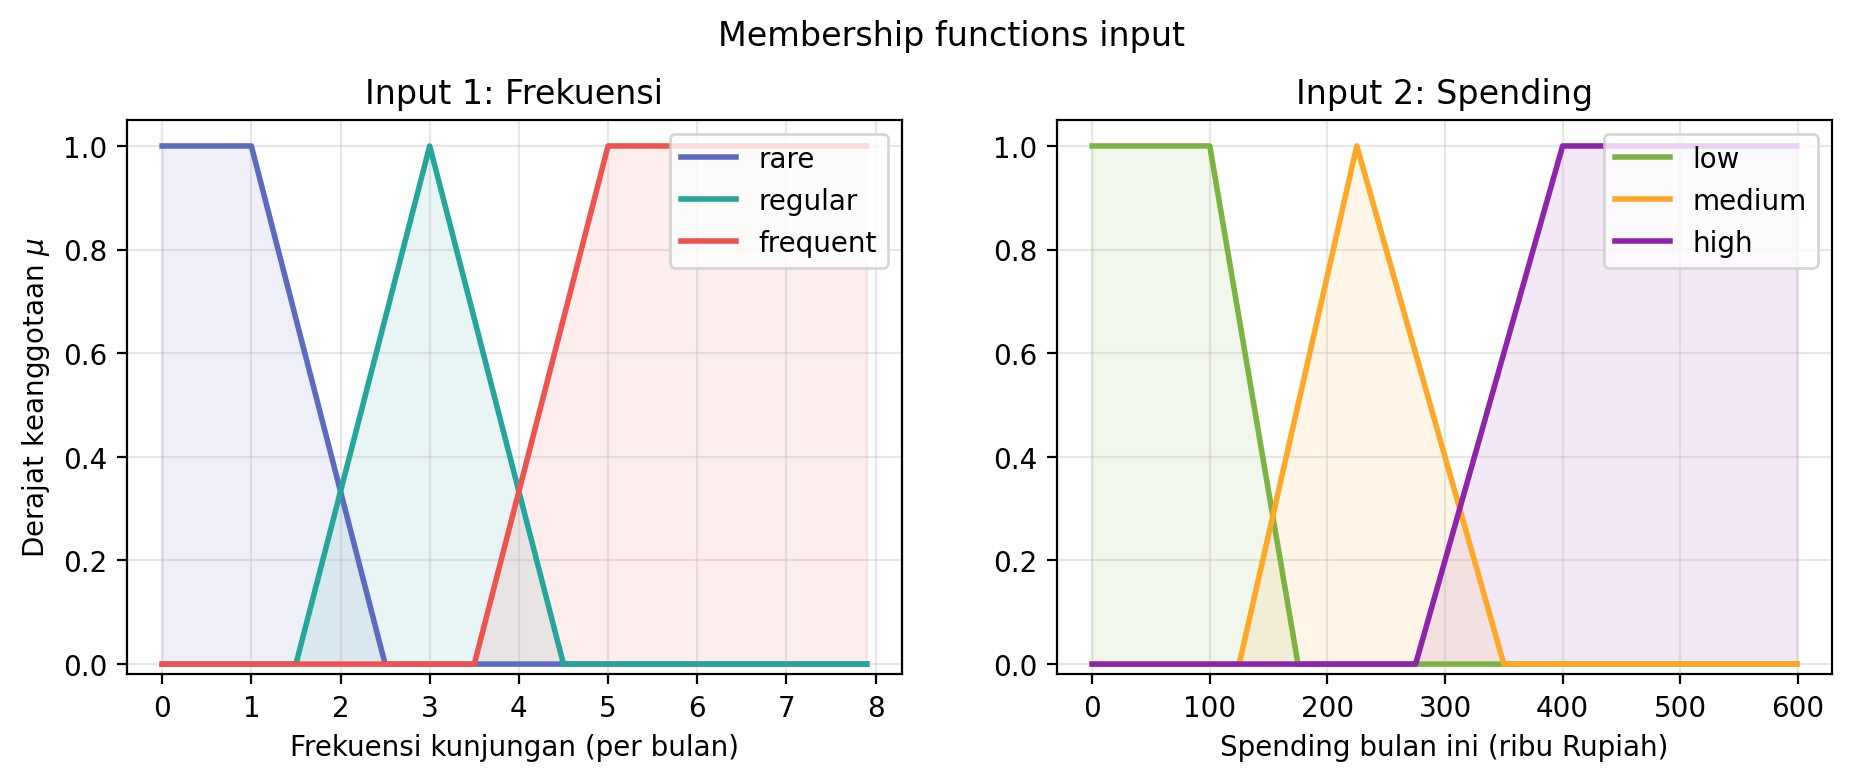
\includegraphics[width=\columnwidth]{mf_inputs.png}
\caption{Membership function dua input. Anchor disesuaikan dengan
tarif barbershop Jakarta 2024--2025.}
\label{fig:mfin}
\end{figure}

\begin{figure}[t]
\centering
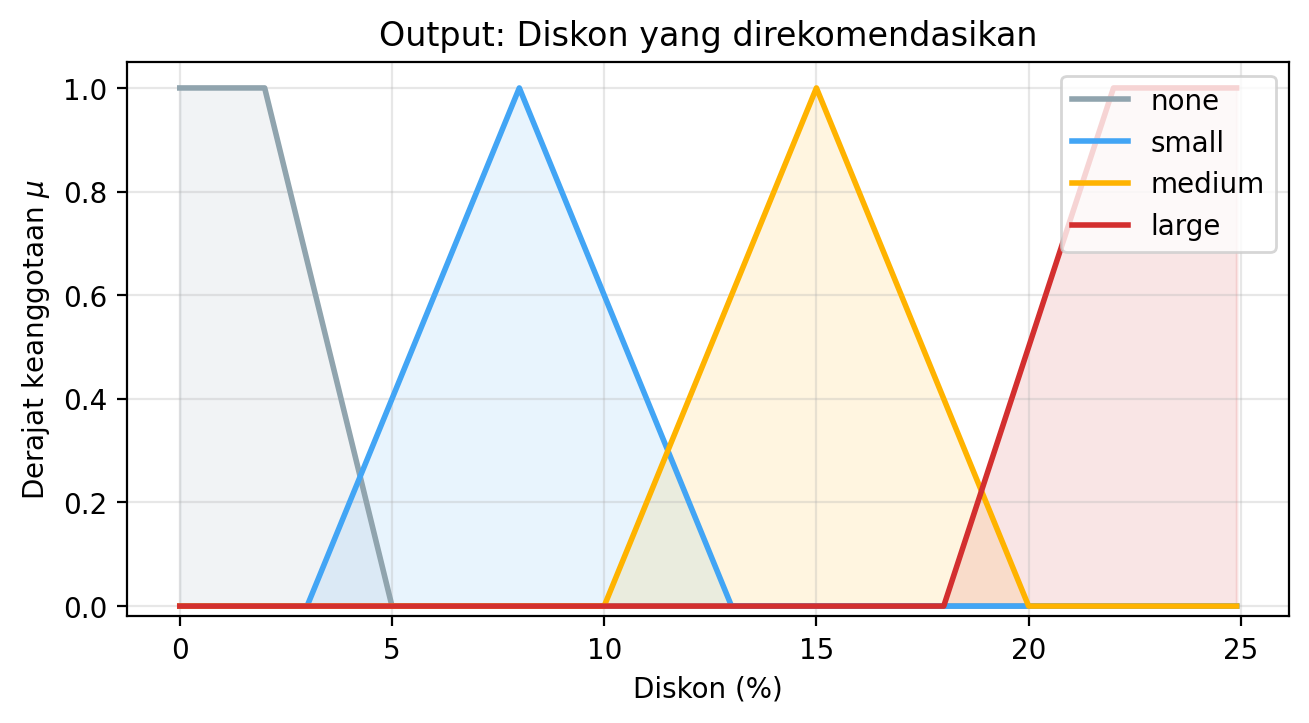
\includegraphics[width=\columnwidth]{mf_output.png}
\caption{Membership function output diskon.}
\label{fig:mfout}
\end{figure}

\subsection{Rule base}

Karena tiap input punya tiga linguistik, saya menerapkan satu aturan
untuk setiap kombinasi. Total ada $3 \times 3 = 9$ aturan, disusun
sebagai grid 3$\times$3 di Tabel~\ref{tab:rules}: sumbu kiri membaca
kategori frekuensi (jarang, sedang, sering), sumbu atas membaca kategori
spending (hemat, standar, premium), dan sel di perpotongannya berisi
kategori output diskon yang harus diberikan untuk profil pelanggan
seperti itu.

\begin{table}[h]
\caption{Sembilan aturan IF--THEN, disusun sebagai grid 3$\times$3.
Sumbu kiri: kategori frekuensi kunjungan. Sumbu atas: kategori spending
bulanan. Setiap sel = satu aturan IF--THEN. Sebagai contoh, sel
(\texttt{rare}, \texttt{high}) berarti aturan ``IF frekuensi
\texttt{rare} AND spending \texttt{high} THEN diskon \texttt{medium}''.}
\label{tab:rules}
\centering
\renewcommand{\arraystretch}{1.1}
\begin{tabular}{l|ccc}
\toprule
\textbf{frekuensi} \textbackslash{} \textbf{spending}
       & \texttt{low}    & \texttt{medium} & \texttt{high}   \\
\midrule
\texttt{rare}     & none   & small  & medium \\
\texttt{regular}  & small  & medium & large  \\
\texttt{frequent} & medium & large  & large  \\
\bottomrule
\end{tabular}
\end{table}

Pola yang saya tanam ke tabel ini ada tiga. Pertama, dari pojok
kiri-atas (\texttt{rare}, \texttt{low}) ke pojok kanan-bawah
(\texttt{frequent}, \texttt{high}), output secara konsisten naik dari
\texttt{none} ke \texttt{large}. Itulah inti aturan loyalti: makin
loyal di salah satu sumbu, makin besar diskonnya. Kedua, sel
diagonal yang ``setara'' (misalnya \texttt{rare}+\texttt{high} dan
\texttt{frequent}+\texttt{low}) sengaja saya beri output yang sama
(\texttt{medium}). Pesannya: pelanggan yang jarang datang tapi
spending besar layak dipertahankan setara dengan pelanggan yang sering
datang dengan spending kecil. Inilah dimensi keadilan multi-dimensi
yang tidak diakomodasi oleh skema bertingkat tradisional. Ketiga, dua
sel sudut kanan-bawah (\texttt{frequent}+\texttt{medium} dan
\texttt{frequent}+\texttt{high}) saya beri output yang sama
(\texttt{large}), sehingga diskon mencapai plateau di pelanggan VIP.
Diskon tidak terus naik setelah pelanggan mencapai profil jelas-jelas
loyal; ini cap operasional supaya margin bisnis tetap aman.

Mari saya bedah baris per baris untuk membuat logikanya konkret.

\textbf{Baris \texttt{rare}} (pelanggan jarang datang) bergerak dari
\texttt{none} ke \texttt{medium} mengikuti spending. Sel
(\texttt{rare}, \texttt{low}) memberi 0\% karena pelanggan baru
(satu kali datang dengan tarif basic) belum perlu insentif --- terlalu
dini untuk diskon, mereka masih dalam fase trial. Sel (\texttt{rare},
\texttt{medium}) memberi \texttt{small} sebagai sinyal apresiasi atas
pilihan layanan yang lebih dari basic. Sel (\texttt{rare},
\texttt{high}) memberi \texttt{medium} --- inilah sel kunci untuk
profil ``eksekutif yang sebulan sekali ambil paket Rp~350k''.

\textbf{Baris \texttt{regular}} (pelanggan dua-tiga kali sebulan)
mengikuti progressi yang serupa, naik satu tingkat dibanding baris
\texttt{rare}: \texttt{small} $\to$ \texttt{medium} $\to$
\texttt{large}. Sel \texttt{(regular, low)} hanya memberi \texttt{small}
karena meskipun pelanggan datang dua kali, dia memilih layanan basic
saja --- masih ada ruang untuk meningkatkan engagement. Sel
\texttt{(regular, medium)} adalah profil ideal pelanggan kantoran
Jakarta yang tipikal, dan saya beri reward standar.

\textbf{Baris \texttt{frequent}} (pelanggan empat kali atau lebih
sebulan) sengaja saya naikkan agresif: bahkan sel
\texttt{(frequent, low)} memberi \texttt{medium}, padahal spending-nya
masih kategori \texttt{low}. Alasannya, biaya operasional barbershop
untuk mempertahankan pelanggan yang sering datang relatif rendah
(setiap kunjungan adalah kunjungan pelanggan eksisting, bukan akuisisi
baru), sehingga reward yang lebih besar tetap aman secara margin.

Sel-sel ini bukan aturan keras yang menghasilkan satu nilai diskrit.
Dalam inferensi Mamdani, satu input yang bukan-eksak akan men-trigger
beberapa sel sekaligus dengan derajat keanggotaan masing-masing. Sebagai
ilustrasi: input frekuensi 2,5 dan spending 200k men-trigger empat sel
secara bersamaan --- (\texttt{regular}, \texttt{low}),
(\texttt{regular}, \texttt{medium}), (\texttt{frequent}, \texttt{low}),
dan (\texttt{frequent}, \texttt{medium}) --- masing-masing dengan
kekuatan firing yang berbeda. Output akhir adalah pusat massa terbobot
dari empat sel itu, dihitung lewat defuzzifikasi centroid pada
sub-bagian berikutnya. Inilah mekanisme yang membuat output fuzzy
halus melewati transisi antar sel, alih-alih melompat dari satu nilai
diskrit ke nilai lain seperti pada skema bertingkat.

\subsection{Inferensi dan defuzzifikasi}

Saya pakai Mamdani min-implication dan max-aggregation. Pemilihan ini
bukan demi akurasi terbaik (Sugeno bisa lebih akurat di kontrol presisi),
melainkan karena setiap aturan harus bisa dibaca pemilik gerai yang
bukan engineer. Defuzzifikasi pakai \emph{centroid of area}, yaitu
pusat massa wilayah hasil agregasi, dihitung diskret di universe
$[0, 25]$ dengan resolusi 0,1\%.

Pilihan ini berimplikasi langsung ke perilaku output. Centroid sensitif
terhadap luas total wilayah aktif, sehingga ketika beberapa aturan
overlap, hasilnya halus melewati batas linguistik. Itulah argumen utama
proposal ini, dan akan saya kuantifikasi pada bagian hasil.

\section{Implementasi}

Implementasi pakai Python 3.12 dengan \texttt{scikit-fuzzy}~0.5.0 sebagai
mesin inferensi, NumPy/pandas untuk numerik dan tabular, Matplotlib untuk
plot, dan Streamlit untuk dashboard. Total kira-kira 320 baris kode
Python tersebar di empat modul utama:

\begin{itemize}
\item \texttt{src/fuzzy.py} --- inti sistem (anchor MF, rule base,
inferensi, defuzzifikasi).
\item \texttt{src/baseline.py} --- skema bertingkat tradisional sebagai
pembanding.
\item \texttt{src/data.py} --- generator 100 profil pelanggan kantoran
Jakarta dari delapan persona.
\item \texttt{src/plots.py} --- pembuat enam figur untuk paper.
\end{itemize}

Listing~\ref{lst:rules} menunjukkan cuplikan pembangunan rule base.
Saya mendeklarasikan rule sebagai kamus
\texttt{(antesedan) $\to$ konsequen}, lalu mengiterasinya ketika membangun
\texttt{ControlSystem}; bentuknya kompak dan rule baru tinggal ditambahkan
satu baris.

\begin{lstlisting}[caption={Cuplikan pembangunan rule base.},label={lst:rules}]
RULE_TABLE = {
    ("rare",     "low"):    "none",
    ("rare",     "medium"): "small",
    ("rare",     "high"):   "medium",
    ("regular",  "low"):    "small",
    ("regular",  "medium"): "medium",
    ("regular",  "high"):   "large",
    ("frequent", "low"):    "medium",
    ("frequent", "medium"): "large",
    ("frequent", "high"):   "large",
}

rules = []
for (f_term, s_term), d_term in RULE_TABLE.items():
    rules.append(
        ctrl.Rule(freq[f_term] & spend[s_term],
                  disc[d_term])
    )
\end{lstlisting}

Untuk demo interaktif saya buat dashboard Streamlit dengan dua slider
input dan tiga tab output: tab Inferensi (badge diskon, MF plot dengan
crisp value), tab Perbandingan (sweep terhadap pembanding), dan tab
Dataset (tabel 100 pelanggan dengan rekomendasi fuzzy sekaligus
pembanding).

Pengujian otomatis pakai \texttt{pytest}, total delapan kasus: dua
boundary (pelanggan baru murni, pelanggan VIP murni), dua monotonisitas
(ke arah frekuensi naik, ke arah spending naik), satu kasus kanonis
(``jarang tapi premium''), satu pengujian rentang output, satu pengujian
struktur dataset, dan satu pengujian eksplisit yang mengukur loncatan di
ambang batas pada skema bertingkat dan memastikan fuzzy halus di titik
yang sama.

\section{Hasil Awal}

\subsection{Beberapa profil contoh}

Tabel~\ref{tab:scenarios} menampilkan lima profil yang sengaja saya pilih
untuk menyentuh sudut-sudut menarik dari ruang input.

\begin{table}[h]
\caption{Hasil sistem fuzzy pada lima profil pelanggan contoh, dibandingkan dengan skema bertingkat.}
\label{tab:scenarios}
\centering
\renewcommand{\arraystretch}{1.1}
\footnotesize
\begin{tabular}{p{0.36\columnwidth} c c r r}
\toprule
\textbf{Profil} & \textbf{freq} & \textbf{spend (k)}
                & \textbf{fuzzy} & \textbf{tier} \\
\midrule
Pekerja baru, basic 1$\times$ & 1 & 90  & 1.9\%  & 0\%   \\
Reguler casual, 2$\times$ basic & 2 & 180 & 11.5\% & 5\%   \\
Eksekutif, paket 1$\times$    & 1 & 350 & 15.0\% & 10\%  \\
Marketing rapi, 3$\times$ cukur+cuci & 3 & 330 & 19.4\% & 10\%  \\
VIP loyal heavy               & 6 & 480 & 22.3\% & 20\%  \\
\bottomrule
\end{tabular}
\end{table}

Baris ketiga (eksekutif, paket Rp~350k 1$\times$) adalah contoh yang saya
maksud di pendahuluan: pelanggan jarang tapi spending besar. Skema
bertingkat menempatkannya di tier menengah (10\%), sedangkan fuzzy
memberi 15\%, karena aturan \texttt{rare AND high $\to$ medium} firing
penuh dengan derajat keanggotaan tinggi pada \texttt{high} (sekitar 0,7
untuk Rp~350k).

Baris keempat menunjukkan kasus kebalikannya. Karyawan marketing yang
sering ketemu klien dan harus tampil rapi, jadi datang tiga kali
sebulan untuk paket cukur dan cuci dengan tarif Rp~110k. Total
spending bulanannya Rp~330k. Pada skema bertingkat dia tetap di tier
menengah (10\%), karena spending bulanannya masih di bawah threshold
Rp~400k. Sistem fuzzy memberi 19,4\% karena aturan
\texttt{regular AND medium $\to$ medium} firing penuh, diperkuat oleh
\texttt{regular AND high $\to$ large} dengan derajat keanggotaan
parsial pada \texttt{high}.

\subsection{Loncatan di ambang batas dihilangkan}

Untuk membuat kelemahan skema bertingkat lebih kasat mata, saya men-sweep
variabel \emph{spending} dari 0 sampai 500k sambil menahan frekuensi
tetap di 2. Hasilnya pada Gambar~\ref{fig:cliff}.

\begin{figure}[t]
\centering
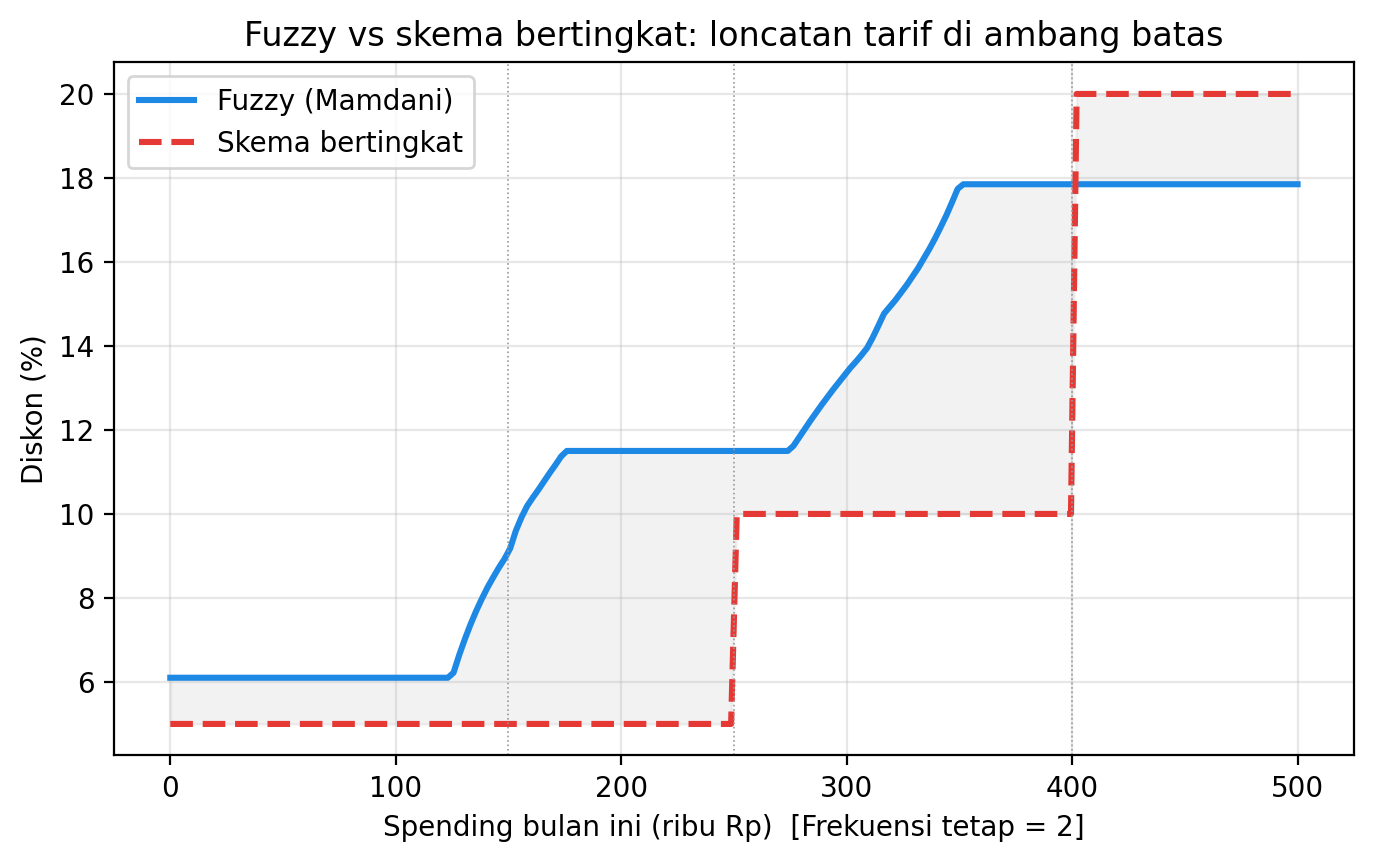
\includegraphics[width=\columnwidth]{fuzzy_vs_baseline.png}
\caption{Diskon sebagai fungsi spending pada frekuensi tetap 2. Garis
vertikal putus-putus menandai tiga ambang batas pada skema bertingkat
(150k, 250k, 400k). Loncatan paling tajam terjadi di Rp~400k, naik 10
poin persentase: pelanggan dengan spending Rp~399k dapat 10\%, sedangkan
pelanggan Rp~400k dapat 20\%.}
\label{fig:cliff}
\end{figure}

Tiga garis vertikal di gambar tersebut adalah ambang batas pada skema
bertingkat. Pada masing-masing ambang ada loncatan: di Rp~150k naik dari
0\% ke 5\%, di Rp~250k naik dari 5\% ke 10\%, dan di Rp~400k naik dari
10\% ke 20\%. Loncatan terakhir adalah yang paling problematis dari sisi
keadilan; selisih Rp~1.000 menggandakan diskon. Kurva fuzzy bergerak
halus tanpa loncatan, melewati tiga ambang itu dengan transisi gradual
yang bisa dibaca sebagai ``loyalitas yang berangsur naik''.

\subsection{Distribusi pada 100 pelanggan kantoran}

Saya generate 100 profil pelanggan dari delapan persona yang umum saya
amati di barbershop Jakarta (entry-level kantoran, reguler casual,
karyawan rapi, profesional muda, eksekutif, VIP, mahasiswa kantor
pinggir, pelanggan Jumatan). Distribusi diskon yang dihasilkan ada di
Gambar~\ref{fig:hist}.

\begin{figure}[t]
\centering
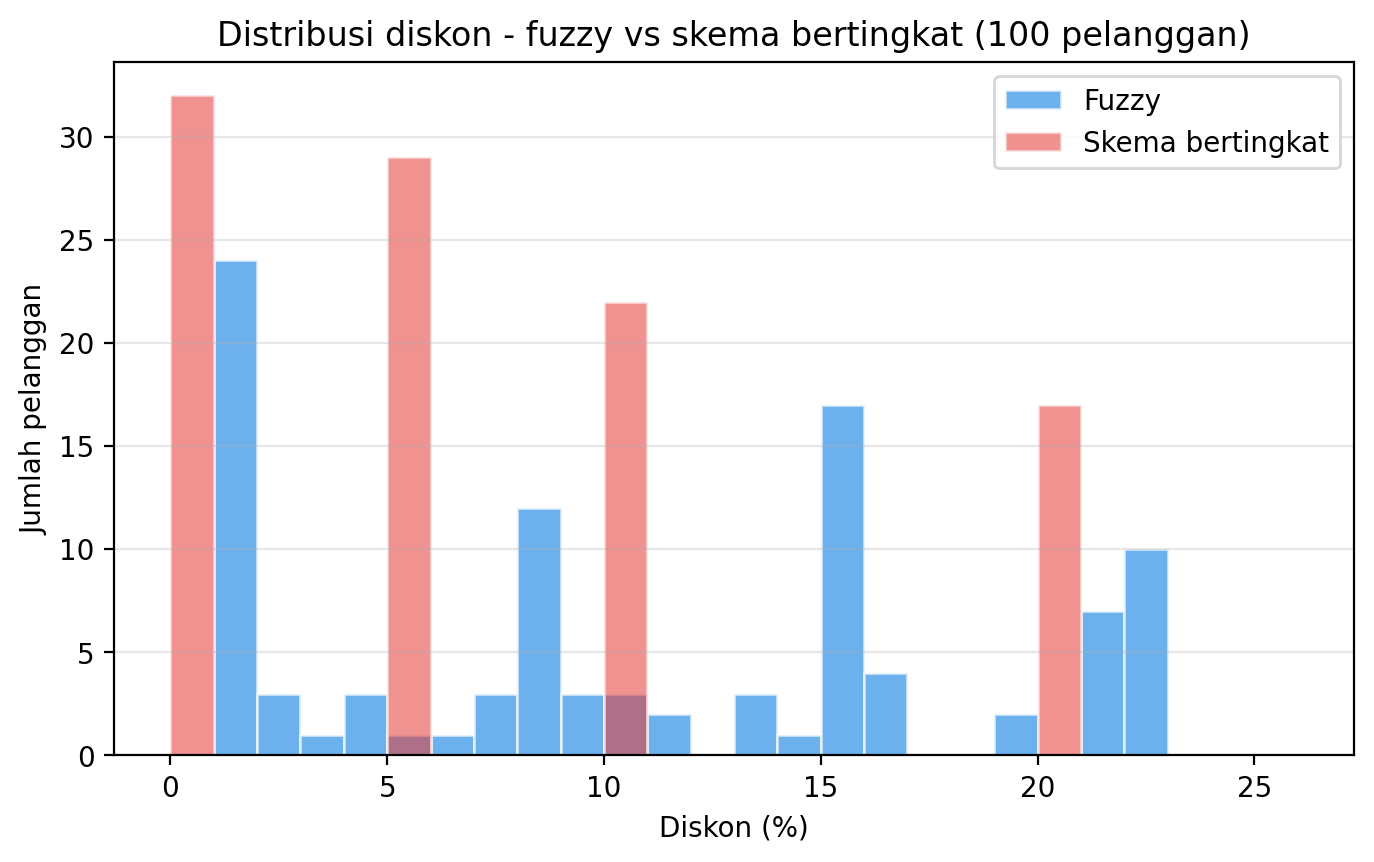
\includegraphics[width=\columnwidth]{disc_distribution.png}
\caption{Distribusi diskon pada 100 pelanggan kantoran. Histogram fuzzy
lebih merata, sementara skema bertingkat hanya mengelompok di empat
titik: 0\%, 5\%, 10\%, dan 20\%.}
\label{fig:hist}
\end{figure}

Yang menarik dari gambar ini: histogram skema bertingkat hanya
mengelompok di empat nilai diskrit (0, 5, 10, 20), karena memang
keluarannya cuma empat angka itu. Histogram fuzzy lebih merata. Itulah
efek interpolasi membership function. Pelanggan dengan profil ``hampir
Silver'' mendapat diskon yang sedikit lebih tinggi daripada Bronze, tanpa
harus melompat penuh ke Silver.

Rata-rata diskon yang direkomendasikan fuzzy untuk 100 pelanggan adalah
10,6\%, sementara skema bertingkat memberikan 9,4\%. Selisih kecil ini
bukan masalah operasional, artinya bisnis yang beralih dari skema
bertingkat ke fuzzy tidak akan mengalami penurunan margin yang berarti.

\subsection{Surface diskon}

Gambar~\ref{fig:surf} menampilkan permukaan diskon di sumbu (frekuensi,
spending). Saya tampilkan ini untuk menegaskan bahwa permukaannya halus
di seluruh ruang input, bukan hanya di garis irisan yang ditampilkan
Gambar~\ref{fig:cliff}.

\begin{figure}[t]
\centering
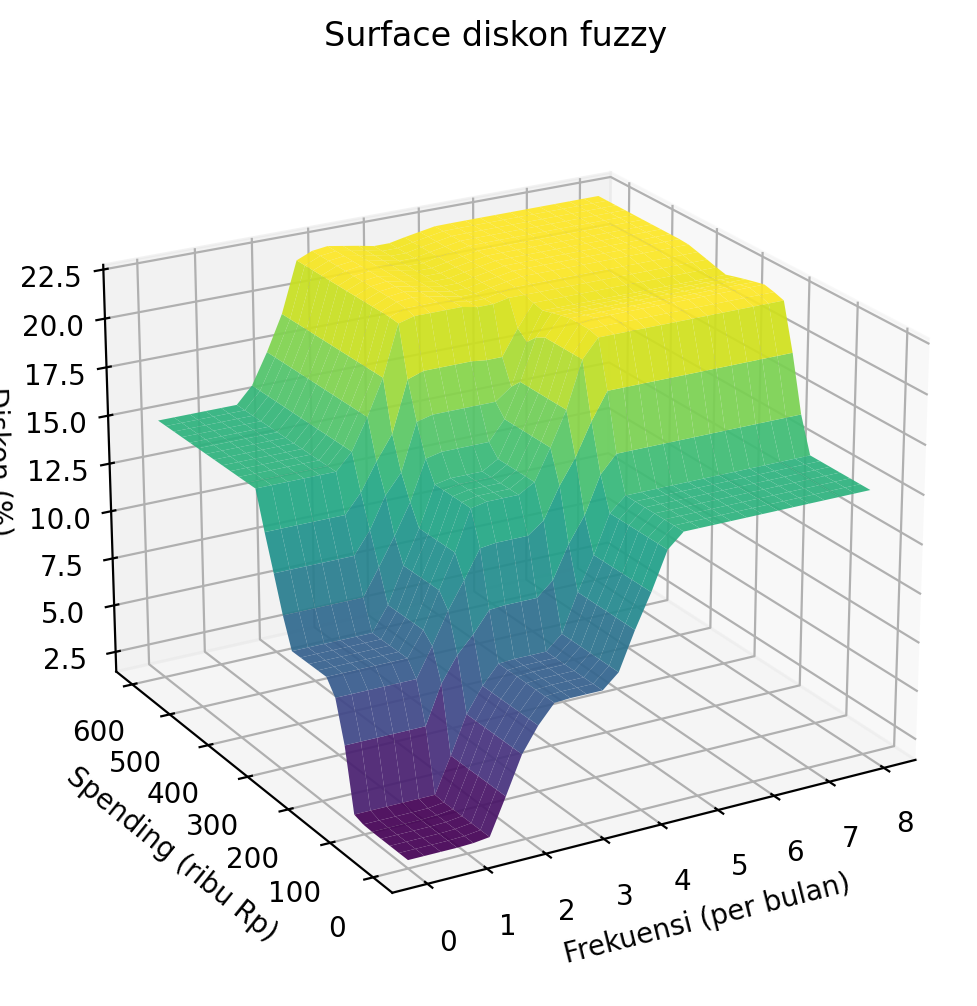
\includegraphics[width=\columnwidth]{surface.png}
\caption{Permukaan diskon fuzzy di sumbu (frekuensi, spending). Naik
monoton ke pojok kanan-belakang, halus di seluruh ruang input.}
\label{fig:surf}
\end{figure}

Sweep ini juga sekaligus berfungsi sebagai sanity check: tidak ada
pelanggan, di mana pun di ruang input, yang akan mendapat diskon turun
saat profil loyalitasnya membaik.

\section{Diskusi}

\subsection{Kekuatan rancangan}

Yang paling saya hargai dari sistem ini adalah \emph{interpretabilitas}-nya.
Sembilan aturan muat di satu tabel 3$\times$3, dan setiap aturan bisa
dijelaskan ke pemilik gerai dalam satu kalimat tanpa istilah teknis. Kalau
pemilik mau mengubah strategi (misalnya tidak lagi memberi diskon untuk
pelanggan \texttt{frequent low} karena dia merasa pelanggan ini sudah
loyal tanpa insentif tambahan), dia bisa langsung mencoret satu sel
di tabel rule.
Tidak perlu retraining model.

Hal kedua, sistem ini tidak butuh data historis pelanggan untuk dipakai
sejak hari pertama. Asumsinya: tarif barbershop tidak banyak berubah dan
profil pelanggan kantoran Jakarta cukup stabil. Sistem berbasis ANFIS atau
generative-baseline butuh data ratusan-ribuan transaksi sebelum bisa
di-deploy; sistem aturan ini bisa langsung bekerja.

\subsection{Keterbatasan}

Yang harus saya akui terlebih dulu: dataset 100 pelanggan adalah
sintetis, dibangun dari delapan persona yang saya susun berdasarkan
pengamatan informal. Ini bukan validasi lapangan. Untuk submission tugas
saya anggap cukup; kalau hendak deployment di gerai nyata, langkah
selanjutnya adalah pengujian A/B selama satu kuarter dengan dua kelompok
kontrol. Aturan yang saya pakai juga belum dituning ke metrik bisnis
tertentu (misalnya retention rate atau average order value).

Keterbatasan kedua, sistem ini stateless. Diskon dihitung dari snapshot
bulan berjalan saja; tidak ada notion ``pelanggan yang baru saja churn''
atau ``pelanggan baru bulan pertama''. Penambahan input ketiga (lama
menjadi member, dalam bulan) bisa menutup celah ini, dengan biaya
membengkaknya rule base ke $3 \times 3 \times 3 = 27$ aturan.

Ketiga, ada asumsi implisit bahwa frekuensi dan spending sama
pentingnya. Pemilik gerai tertentu mungkin punya prioritas berbeda,
misalnya prefer pelanggan high-spending walaupun jarang. Untuk kasus
seperti itu, rule base bisa di-skew (lebih banyak \texttt{large} untuk
profil spending tinggi), tanpa harus mengubah arsitektur sistemnya.

\subsection{Rencana pengembangan}

Beberapa hal yang saya antri kerjakan setelah submission: integrasi
langsung ke POS gerai (membaca transaksi real-time, mengeluarkan diskon
di voucher); penambahan input ketiga ``durasi sebagai member''; A/B test
dengan satu cabang selama 90 hari; dan visualisasi histori diskon per
pelanggan untuk memantau perilaku setelah mendapat insentif.

Untuk kebutuhan akademis, saya juga ingin menjajaki Sugeno first-order
sebagai pembanding numerik. Saya menduga Mamdani akan tetap menang dari
sisi interpretabilitas di domain ini, tapi pembanding angka tetap
bermanfaat sebagai validasi pilihan formulasi.

\section{Penutup}

Saya merancang dan mengimplementasikan sistem fuzzy Mamdani sederhana
untuk merekomendasikan diskon loyalti barbershop. Sistemnya kecil
(sembilan aturan, dua input, satu output) tetapi cukup untuk
menyelesaikan dua masalah konkret pada program loyalti yang umum dipakai
di Jakarta: loncatan tarif di sekitar ambang batas, dan ketidakadilan
terhadap pelanggan dengan profil multi-dimensi. Hasil prototipe pada 100
pelanggan sintetis menunjukkan kurva diskon yang halus melewati seluruh
ruang input, dan kemampuan untuk memberikan apresiasi proporsional ke
kasus seperti ``eksekutif yang jarang datang tapi spending tinggi''.
Kode sumber dan dataset tersedia di repository publik dengan harapan
bisa dipakai-ulang oleh pemilik gerai lain.

\section*{Reproducibility}
Source code dan dataset dirilis di repository publik:
\textbf{\url{https://github.com/ibnubt/fuzzy-barbershop-loyalty}}.
Cara replikasi: install dependensi via \texttt{requirements.txt}, lalu
jalankan \texttt{python -m src.data} (generate dataset),
\texttt{python -m src.plots} (regenerasi figur), \texttt{pytest tests/}
(uji), atau \texttt{streamlit run app/dashboard.py} (dashboard).

\bibliographystyle{IEEEtran}
\bibliography{references}

\end{document}
